

\chapter{Konzeptionierung einer integrierten Python Anwendung}\label{PythonApp}

Die Basisanforderungen einer integrierten LZ-Verwaltung lassen sich aus Kapitel \ref{Kap2} ableiten.
Hinzu kommen die später in Kapitel 5 beschriebenen Funktionen.
Anhand dieser beiden Punkte kann man erkennen, dass Modularität, Erweiterbarkeit sowie Wartbarkeit wichtige Kriterien sind.
Darüber hinaus müssen diese Schritte auch von Personen durchgeführt werden können, die mit der ursprünglichen Entwicklung
der Software nicht involviert waren.
Eine saubere Struktur der Software ist dazu unerlässlich.
Die alte Software nutzte eine GUI-Klasse als Datenhub.
Dadurch entstand ein unübersichtliches Klassenkonstrukt, dass es schwer machte sich in den Code zu überschauen.
Zum Beispiel wird anhand der Klassendiagramme deutlich, dass Daten der Modbus Adressen in die \verb|commissionMatrix|
geschrieben werden müssen, weil sie ausschließlich dort zu RAPID Kommandos für den Industrieroboter übersetzt werden.
Wie genau das passiert, lässt sich jedoch anhand des C\# Codes nicht nachvollziehen.
Mit einer Menge Zeitaufwand könnte dieses Rätsel aufgelöst werden, jedoch bringt es für die Konzeptionierung der neuen
Software keinen Mehrwert.\\
\vspace{1cm}
Um solche Unannehmlichkeiten für die Zukunft zu vermeiden, empfiehlt es sich auf branchenübliche Design Patterns
zurückzugreifen.
Dieses MVC Konzept sieht vor, dass Daten (Model) und GUI (View) keinerlei Zugriff aufeinander erlauben.
Die Schnittstelle zwischen den Daten und dem Benutzer ist ein Controller, der die Programmlogik implementiert.
Für die Daten gilt, dass sie in einer Objektstruktur modelliert werden und nicht von außerhalb dieser Objekte verändert
werden.
\vspace{1cm}
Soll das Datenmodell gerändert werden, muss dafür eine öffentliche Methode in dem Modell selbst existieren,
die alle möglichen Fehler abfängt und referenzielle Integrität herstellt, sodass das Datenmodell nach jeder berechtigten
Änderung konsistent bleibt und unberechtigte Änderungen nicht zulässt.\\
Die drei Klassen in Abb. \ref{fig:figure9} besitzen private Attribute, was durch das \glqq - \grqq angedeutet ist.
Dafür besitzen sie öffentliche Methoden, die einerseits die Attribute zurückgeben (get-Methoden) oder einen zu verändernden
Wert übernehmen (set - Methoden).
Werden Listen verwendet, können Objekte mit den with- und without - Methoden hinzugefügt oder entfernt werden.
Ein Objekt der Klasse \verb|Pallet| kann sich also nicht direkt selbst in das entsprechende Feld eines Objekts der Klasse
\verb|Cup| eintragen, sondern muss dazu die entsprechende Methode \verb|SetPallet()| aufrufen.
Diese Methode muss mindestens die folgenden Kriterien erfülllen um referenzielle Integrität herzustellen:
Erstens muss die Gültigkeit der übergebenen Parameter geprüft werden.
Zweitens muss überprüft werden ob in dem zu schreibenden Attribut schon ein anderes Objekt vermerkt ist.
Drittens müssen die Änderungen jeder betroffenen Klasse mitgeteilt werden und eventuelle Fehlerfälle behandelt werden.
Wird zum Beispiel einem Objekt der Klasse \verb|Cup| je ein Objekt der Klasse  \verb|Pallet| und \verb|Product|
übergeben, dann muss am Ende der Änderung das \verb|Cup| Objekt in der Liste \verb|cups| der Klasse \verb|Product| stehen.
Das Objekt der Klasse \verb|Pallet| muss ebenfalls als Feldwert des Attributs \verb|cup| das Objekt der \verb|Cup| Klasse haben.\\

\vspace{1cm}
\begin{figure}
        \caption[Beispiel: Referenzielle Integrität]
        {\small Refrenziellen Integrität einer Palette / Becher / Produkt - Kombination wie sie in der $\mu$Plant
        auftreten könnte. }\label{fig:figure9}
        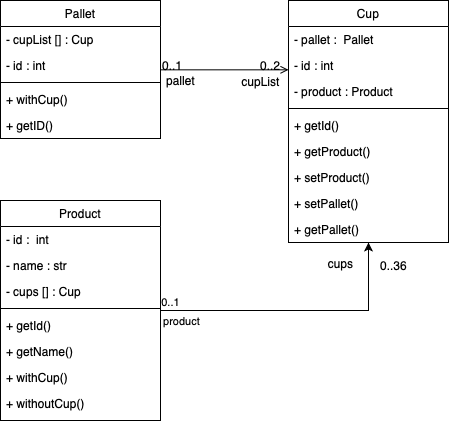
\includegraphics[width = \textwidth ]{Bilder/BeispielRefInt}
        \centering
\end{figure}

\newpage
\section{PySide6 und QuickQml 2.0}

Laut der Qt Wiki Website \cite{QtWikiHistory} wurde das Qt Framework geboren als ihre Schöpfer Haavard Nord und
Eric Chambe-Eng im Sommer 1990 in Norwegen an einem GUI für eine Ultraschalldatenbank arbeiten.
Die Software sollte damals in C++ implementiert auf Mac, Unix und Windows laufen.
Fünf Jahre später veröffentlichten Sie das erste Qt Framework unter dem Firmennamen Troll Tech.
Seitdem gewann das Framework immer mehr Popularität.
Im Jahr 2006 übernahm Nokia die Firma Troll Tech und verkaufte das Qt Project in den Jahren 2011 und 2012 erst teilweise,
dann vollständig an den Digia Konzern.
Seit 2014 ist Qt als Tochterunternehmen des Digia Konzerns unter dem Namen \glqq The Qt Company\grqq ein eigenständiges Unternehmen.

Das Qt Framework ist in C++ implementiert.
Die neue Software für die $\mu$Plant soll jedoch in Python implementiert werden.
Für diese Zwecke hat Qt u.A. das Framework PySide6 veröffentlicht, welches einen Wrapper für Python Projekte bietet.

GUI's können in PySide6 im Wesentlichen auf zwei Arten erstellt werden.
Eine Möglichkeit ist es, das GUI über Widgets\cite{pysideQtWidgets} zu erstellen, die direkt im Python Code implementiert werden können.
Die zweite Möglichkeit ist QtQuick \cite{pysideQtQuick} zu nutzen, bei dem das GUI in einer separaten QML Datei erstellt wird und
mittels einer \verb|QtQmlApplicationEngine| Klasse in das Programm eingebunden wird.

Für die Umsetzung eines MVC-Design Patterns empfiehlt sich die Verwendung von QtQuickQML.
Durch die Verwendung des Frameworks wird die konsequente Trennung zwischen Interface und Datenmodell erzwungen.
Veranschaulicht wird dies in Abb. \ref{fig:figure10}.
Die eigentlichen Daten (von Server oder Datei) werden in ein Datenmodell (Model) überführt.
Dieses Datenmodell ist ein beliebig komplexes Klassenkonstrukt, welches referenzielle Integrität aufbaut.
In Pyside6 muss dieses Datenmodell von der Basisklasse \verb|QAbstractModel| abgeleitet werden.
Beim Initialisierung der Anwendung wird eine Instanz dieser Klasse (oder einer abgeleiteten Klasse) erstellt und als
Root-context der \verb|QQmlApplicationEngine| registriert.
Somit ist das Datenmodell mit dem GUI verknüpft und kann unter seiner URI in jedem QML File angesprochen werden.
In einer QML Datei wird ein entsprechender QML Type, z.B. \verb|ListView|, welches eine einfache Liste erzeugt,
und dem Property \verb|model| die URI des Datenmodells zugewiesen.
Dadurch kennt das \verb|ListView| Objekt die Indices des Datenmodells und erhält beim Rendern der Liste nur die benötigten
Daten.
Jede weitere Aktion, die durch den Benutzer auf ein Listenelement ausgelöst wird, bezieht sich auf ein Delegate des Datenmodells.
Jede Änderung an dem Delegate wird zunächst gerendert und überprüft bevor das Datenmodell geändert wird.
Diese Basisfunktion kommt mit dem Qt Framework an sich und muss nicht implementiert werden.
Wie jedoch das Datenmodell mit den geänderten Daten umgeht oder ob die Änderung des Datenmodells automatisch ein Update
der Daten auf dem Server oder der Datei auslöst, muss vom Entwickler implementiert werden!
An ein Delegate sind je nach QmlType durch das Framework Signale gebunden.
Signale sind Teil des Signal/Slot Prinzips des Qt Framework \cite{pysideSignalSlot} und stellen die Funktion eines Events dar.
Durch die \verb|QmlApplicationEngine| sind innerhalb eines GUIs alle Root-context Elemente ansprechbar.
Wird ein Signal an beliebiger Stelle im GUI emittiert, kann es an jeder anderen Stelle als Event genutzt werden.
Dadurch muss man  in der Regel keine zusätzlichen Callbacks oder Lamda-Ausdrücke definieren.
Außerhalb des QML Contexts, z.B. in einer Python Klasse, muss das Signal der Klasse bekannt sein, indem das Signal an die Klasse
gebunden wird.
Eine Funktion die mit der Annotation \glqq Slot(str) \grqq versehen ist, wird als Slot behandelt und kann mit dem Signal
verknüpft werden, sodass diese bei Auftreten des Signals ausgeführt werden.
An Signale können Daten übergeben werden, die so in einem Slot weiterverarbeitet werden können.\\
\vspace{1cm}
In meiner Vorbereitung auf diese Arbeit hat sich eine intuitive Vorgehensweise entwickelt, die ich für die Implementierung
der Software empfehlen möchte:\\
\vspace{1cm}
Beim Initialisieren des Programms werden alle Datenmodelle (\verb|QAbstractModel| und abgeleitete Klassen), Controller
und Serviceklassen instanziert und als Root-context der \verb|QQmlApllicationEngine| gesetzt.
Siehe dazu das Beispiel \ref{exampleApp}.
Damit stehen sie dem Programmierer in jeder QML Datei der Anwendung zur verfügung.\\
In einer QML Datei können die Kontexte der QQmlEngine nun unter ihrer URI referenziert werden.
Dies ist in Beispiel \ref{exampleListview} gezeigt:\\
In dem QML Type \glqq ListView \grqq wird dem Property \verb|model| die URI des listModels aus \ref{exampleApp} zugewiesen.
Im weiteren Verlauf des Codes findet sich ein \verb|MouseArea| QML Type.
Wird in dem Bereich ein Klick mit linker Maustaste durchgeführt, wird das Signal \verb|onClicked| emittiert.
Innerhalb des \verb|MouseArea| Codes wird definiert, dass nach einem Mausklick die Funktion \verb|selectRow(message)|
aufgerufen wird. \verb|message| ist dabei der übergebene Parameter.
Das Beispiel braucht dabei keinerlei Importe anderer Klassen, was daran liegt, dass sowohl das DatenModell als
auch das Objekt der Controller Klasse als Ressource der QQmlEngine registriert wurden.
Im weiteren Verlauf des Codes wird ein QML Type \verb|Connections| erzeugt, bei dem das Signal des Controllers \verb|onRowClicked|
mit einer Funktion verbunden wird.
Innerhalb des \verb|Connections| Types wird in Javascript die Funktion definiert.
Zu beachten ist, dass im Controller selbst das Signal als \verb|RowClicked| definiert wird.
Innerhalb der QML Datei werden die Signale dann mit dem Präfix \glqq on \grqq erfasst.
Der Signalname wird als Name einer javascript - Funktion verwendet, die mit \verb|function| gekennzeichnet ist.
Der Code innerhalb des Funktionskörpers beschreibt dann die Funktionslogik in Javascript.
Im Fall des Beispiels wird ein bool'sches Property umgeschaltet, wenn die \verb|id| des Datenmodell - Delegates mit der
\verb|message| des Signals übereinstimmt.

\lstset{
    basicstyle=\small\ttfamily
}
\newpage
\lstinputlisting[language=Python,
        caption ={Beispiel einer einfachen App mittels PySide6. \small Zunächst wird eine Instanz der
Application-Klasse und der QmlEngine erzeugt. Danach werden Objekte eines Datenmodells und
eines Controllers erzeugt und als rootContext der QmlEngine registriert. Anschließend wird die QML Datei des Hauptfensters geladen,
was die App startet.}]
{Listings/Demo1.py}\label{exampleApp}

\lstinputlisting[language=xml,
caption ={Beispiel einer QML Datei\small Diese QML Datei erzeugt ListView QML Type, der zum Anzeigen der Daten
in einem ListModel verwendet wird. Innerhalb eines Rechtecks mit farbigem Rand werden in einem RowLayout Type die
Datensätze des Datenmodells gerendert und über die Funktionslogik von Signalen der QML Types und der Controllerklasse
farblioch markiert.}]{Listings/listviewExample.qml}\label{exampleListview}
\newpage

\begin{figure}
        \caption[Model-View Konzept mit zusätzlichem Controller und Service ]
        {\small Die Abbildung zeigt das in PySide6 verwendete Model-View Konzept, welches um einer Controllerklasse und
        einer Service Klasse erweitert wurde. }\label{fig:figure10}
        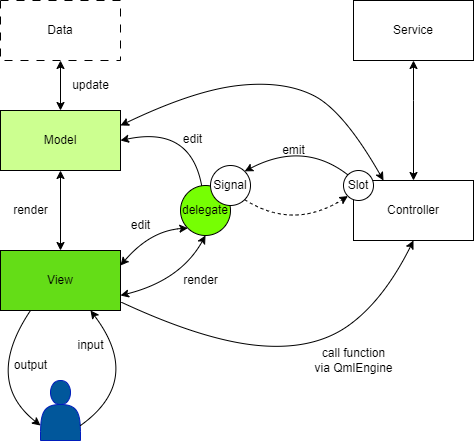
\includegraphics[width = \textwidth ]{Bilder/MVCS_Beispiel}
        \centering
\end{figure}

\newpage

Aus den Beispielen \ref{exampleApp} und \ref{exampleListview} lässt sich eine Systematik erkennen:
Die Daten sind hinter einem DatenModel geschützt und werden der View zur Verfügung gestellt.
Über die QML Dateien erfolgt die GUI Modellierung und Events werden mit dem Signal/Slot Prinzip behandelt.
Beliebige Ressourcen können als Teil der QmlEngine registriert werden, um Sie an anderer Stelle verfügbar zu machen.
Das künftige Programm soll jedoch auch Programmteile aufweisen, die nicht unbedingt mit den Daten oder dem GUI verknüpft sind.
Das sind beispielsweise die Kommunikationen über ModBus und dem ABB Industrieroboter oder das Übersetzen der Modbus Werte in
RAPID Befehle.
Diese Programmteile werden als Service Klassen bezeichnet.
Wenn sich der Programmcode auf ein GUI auswirkt, wird ein Controller gebraucht, der dieses Verhalten steuert.
Selbstverständlich könnten die Funktionen eines Controllers in den Service integriert werden.
Dies würde aber die Wartbarkeit und Erweiterbarkeit verschlechtern.
Nach der Systematik wie in \ref{fig:figure10} abgebildet, können beliebig viele Datenmodelle, GUI's, Controller und Services
parallel existieren ohne sich gegenseitig zu beeinflussen.\\
Als Nachteil kann angeführt werden, dass sich mit zunehmendem Kontextregister der QmlEngine die Performance des Programms
verschlechtern wird.
Bei dem eher gering erwarteten Funktionsumfang der zu erstellenden Software ist dies jedoch untergeordnet und könnte
durch das dezidierte Aufteilen der Funktionen in Threads reduziert werden.

\section{GUI - Konzeptionierung}

Die Hauptfunktion der Software war bisher das automatisierte Abarbeiten der Kommissionsaufträge, die über Modbus TCP/IP
von der Auftragsverwaltung der $\mu$Plant übergeben werden.
Während diese Funktion abläuft, macht der Benutzer höchstwahrscheinlich einen Soll-Ist-Vergleich zwischen dem GUI
und dem was er in der LZ sieht.
In Abb. \ref{fig:figure11} ist ein Entwurf dargestellt welche Elemente sichtbar sein sollten, wenn der Automatikbetrieb läuft.
Links ist die Andockstation des mobilen Roboters simuliert mit einem RFID Gerät darüber [Fehlt noch eine zufriedenstellende Idee wie die Daten des RFID Readers angezeigt werden].
Der Kommissioniertisch ist mit seinen beiden Plätzen \glqq K1 \grqq und \glqq K2\grqq  daneben symbolisiert.
Die Visualisierung des Lagers nimmt den gesamten rechten Bildschirm ein.
Die Produktliste, wie sie in \ref{fig:figure} Bereich \glqq D\grqq dargestellt ist, kann entfallen.
Muss der Bediener ein Produkt an irgendeiner Stelle des Programms überschreiben, so wird ihm nicht mehr die Produkt ID
angezeigt, sondern direkt der Name.
Zusätzlich könnte die Produktliste als Neues Fenster auf Wunsch des Benutzers eingeblendet werden.
Zum Beispiel über die Toolbar.
Sämtliche Einstellungen wie Ip und Port der Kommunikationsschnittstellen sollen nur bei Bedarf angezeigt werden.
Ihr Aufruf soll über die Toolbar erfolgen.
Die Bereiche \glqq E\grqq (Inventarliste) und \glqq F\grqq (Eventlog) aus Abb \ref{fig:figure} Müssen nicht
gleichzeitig sichtbar sein.
Sie können in einem Register integriert werden und mit dem QML Type \verb|StackView| oder einem Loader angezeigt werden.
Das Erscheinungsbild der beiden GUI Elemente kann aus der alten Software übernommen werden.
Als Drittes Register soll zusätzlich zum alten Startbildschirm eine Commission List hinzugefügt werden.
Sie soll eine Übersicht über die von der Auftragsverwaltung eingetroffenen Aufträge und ihren Status anzeigen.
Um Manuelle Überschreibungen der Produkte und Cup IDs vorzunehmen, ist vorgesehen, dass ein Zahnrad-Symbol erscheint,
wenn man über dem entsprechenden Bereich den Mauszeiger hält (Hovering).
Bei Klick auf das Zahnrad-Symbol soll ein Objekt des QML Types \verb|QDialog| eingeblendet werden in dem die alten
Feldwerte angezeigt und editiert werden können, aber auch das Editieren verworfen werden kann.\\
\vspace{1cm}

Die Funktion des Controllers soll über die Toolbar aufgerufen werden.
Der Begriff an sich ist im Zusammenhang mit der neu konzipierten Software irreführend und wird daher verworfen.
Der Oberbegriff \glqq Manual Processing \grqq wird stattdessen gewählt.
Hiermit sollen manuell Transportaufträge erzeugt werden wie \glqq Räume den Becher aus Lagerort L3a nach L6b \grqq.
Im Grunde soll dies für jede denkbare Operation möglich sein.
Bei Klick auf den entsprechenden Eintrag in der Toolbar könnte sich ein Fenster oder ein Dialog öffnen wie in
\ref{fig:figure12}.
Die so neu erzeugten Transportaufträge werden ebenfalls in der Commission List angezeigt.

\begin{figure}
        \caption[Mockup des Startbildschirms]
        {\small Die Abbildung zeigt wie der Startbildschirm aussehen könnte um die Funktion des Automatikbetriebs abzubilden:
        }\label{fig:figure11}
        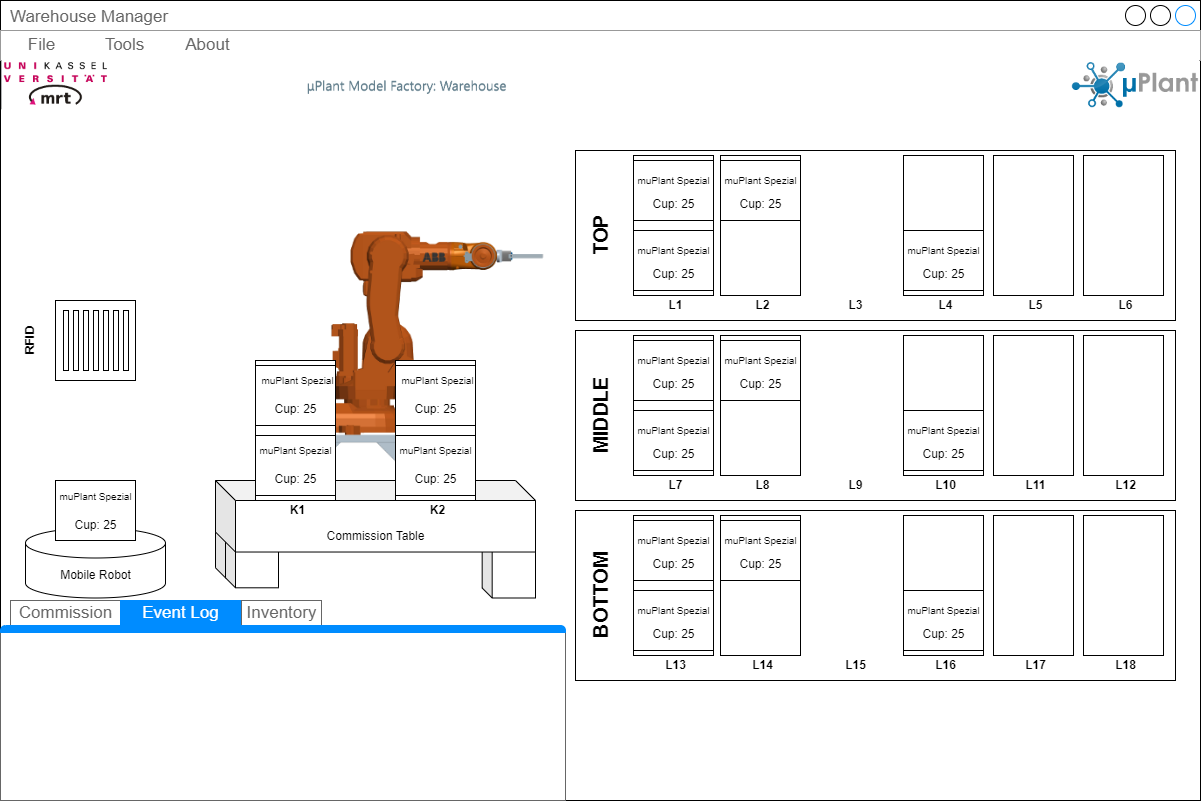
\includegraphics[width = \textwidth ]{Bilder/Mockup_Startbildschirm}
        \centering
\end{figure}

\begin{figure}
        \caption[Mockup des Menüs für die Manuelle Lagersteuerung]
        {\small Die Abbildung zeigt, dass entweder ein Becher oder eine Palette (mit oder ohne Becher) vom Startort zum
        Zielort transportiert werden kann. Die Eingabe der Zielorte wird hier über zwei Dropdown Menüs realisiert.
        Das Mockup impliziert, dass bei Tätigung einer Eingabe eine Validierung der Eingaben erfolgt.
        }\label{fig:figure12}
        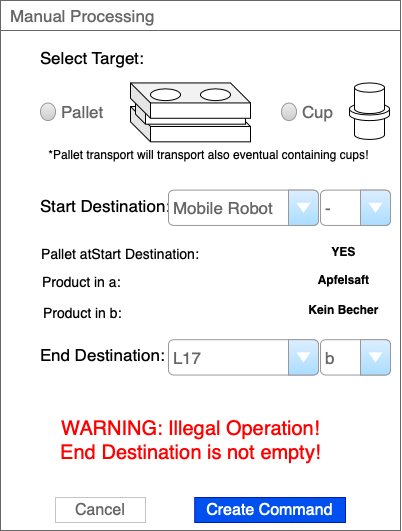
\includegraphics[width = \textwidth ]{Bilder/Mockup_ManualProcessing}
        \centering
\end{figure}


\section{Konzepte zur Datenmodellierung}

\section{Konzepte für Controller- und Serviceklassen}

\section{Teilautomatisierte Code Dokumentation}